% \iffalse
\let\negmedspace\undefined
\let\negthickspace\undefined
\documentclass[journal,12pt,twocolumn]{IEEEtran}
\usepackage{cite}
\usepackage{amsmath,amssymb,amsfonts,amsthm}
\usepackage{algorithmic}
\usepackage{graphicx}
\usepackage{textcomp}
\usepackage{xcolor}
\usepackage{txfonts}
\usepackage{listings}
\usepackage{enumitem}
\usepackage{mathtools}
\usepackage{gensymb}
\usepackage{comment}
\usepackage[breaklinks=true]{hyperref}
\usepackage{tkz-euclide} 
\usepackage{listings}
\usepackage{gvv}                                        
\def\inputGnumericTable{}                                 
\usepackage[latin1]{inputenc}                                
\usepackage{color}                                            
\usepackage{array}                                            
\usepackage{longtable}                                       
\usepackage{calc}                                             
\usepackage{multirow}                                         
\usepackage{hhline}                                           
\usepackage{ifthen}                                           
\usepackage{lscape}
\usepackage{tabularx}

\newtheorem{theorem}{Theorem}[section]
\newtheorem{problem}{Problem}
\newtheorem{proposition}{Proposition}[section]
\newtheorem{lemma}{Lemma}[section]
\newtheorem{corollary}[theorem]{Corollary}
\newtheorem{example}{Example}[section]
\newtheorem{definition}[problem]{Definition}
\newcommand{\BEQA}{\begin{eqnarray}}
\newcommand{\EEQA}{\end{eqnarray}}
\newcommand{\define}{\stackrel{\triangle}{=}}
\theoremstyle{remark}
\newtheorem{rem}{Remark}
\begin{document}
\bibliographystyle{IEEEtran}
\vspace{3cm}

\title{NCERT-discrete : 10.5.3 - 2}
\author{EE23BTECH11025 - Anantha Krishnan $^{}$% <-this % stops a space
}
\maketitle
\newpage
\bigskip



\section{question}
\vspace{0.5cm}
Find the sums given below:
\begin{enumerate}
    \item[(i)] 7 + $10\dfrac{1}{2}$ + 14 ... + 84
    \item[(ii)] 34 + 32 + 30 ... + 10
    \item[(iii)] -5 + -8 + -11 ... -230

\end{enumerate}

\vspace{0.5cm}
\textbf{Solutions}:
\begin{enumerate}
\item[(i)]   
7 + $10\dfrac{1}{2}$ + 14 ... + 84\vspace{0.05cm}
\vspace{0.2cm}

Let $S_i{(k)}$ denote the sum of first k terms in the $i^{th}$ series , $x_i(0)$ denotes its first term , $d_i$ denotes the common difference and $u_{(k)}$ denote thte unit step function.
\begin{align}
{S_k} = \dfrac{ku_{(k)}}{2}(2x_i(0) + (k-1)d_i)\label{eq:1}
\end{align}
For number of terms , we use
\begin{align}
x_i(n) = (x_i(0) + nd_i)u_n\label{eq:2}
\end{align}
Where $x_i(n)$ is the $(n+1)^{th}$ term of the series. Putting the values
\begin{align}  
84 = 7+\dfrac{7n}{2}\\
n=22
\end{align}
\item 
\textbf{Calculating $S_1(k)$ for $x_1(n)$} : 
We now use this result for calculating $S_1(23)$
\begin{align}
    S_1{(23)} = \dfrac{23}{2}(14+(22)\dfrac{7}{2})
    \end{align}
Solving this yields $S_1{(23)}$ = 1046.5\vspace{0.05cm}\vspace{0.05cm}
We are now required to calculate $X_1(z)$ in terms of $u_n$ and $x_1(n)$.Where u$_{(n)}$ is the unit step function.
\begin{align}
    x_1(n) = u_{(n)}(x_1(0)+\dfrac{7n}{2})
    \end{align}
    \begin{figure}[!ht]
    \centering
\graphicspath{ {figs/} }
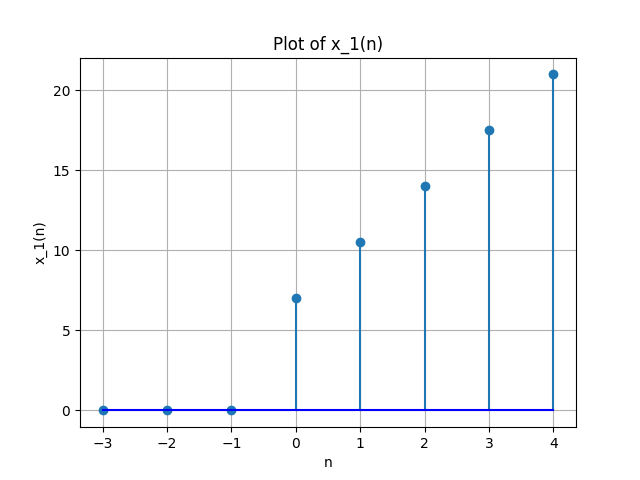
\includegraphics[width=10cm, height=6cm]{graph_1}
\captionsetup{Graph:1 $x_1(n)$ vs n }
\end{figure}
\vspace{0.05cm}
\item 
\textbf{Z-Transform of $x_1(n)$} :
\vspace{0.2cm}
By the Definition of Z-transform:
\begin{align}
 \sum_{n=-\infty}^{\infty} Z^{-n}x_i(n) = X_i(Z)\label{eq:3}
 \end{align}
\vspace{0.05cm}Putting $x_1(n)$ in $\eqref{eq:3}$ , we get \vspace{0.05cm}
\begin{align}
     \sum_{n=-\infty}^{\infty}(x_1(0) + \dfrac{7n}{2})u_{(n)}Z^{-n} =X_1(z)
\end{align}
\begin{align}
\sum_{n=-\infty}^{\infty}(7 + \dfrac{7n}{2})u_{(n)}Z^{-n} =X_1(z)
\end{align}
\begin{align}
\notag7z(1-z)^{-1}+\\
\notag 7z((1-z))^{-1}+\\
7z(2(1-z))^{-2}=X_1(z)
\end{align}
\vspace{0.05cm}
\vspace{0.05cm}
\item[3)]
\textbf{Region of Convergence}
\vspace{0.05cm}
\begin{align}
    \lvert z\rvert  <  1 
    \end{align}

\vspace{1cm}

\vspace{0.5cm}
\item[(ii)]
 34 + 32 + 30 ... + 10\vspace{0.05cm}
\vspace{0.2cm}

In this bit  $x_2(0)$ = 34 , $d_2$ = -2.\\

Using equation \eqref{eq:2}
\begin{align}
     10 = 34 -2n\\
     n=12 
     \end{align}
For $x_2(n)$
\begin{align}
x_2(n) = x_2(0) + nd_2\\
x_2(n) = x_2(0) -2n
\end{align}

\begin{figure}[!ht]
\centering
  \graphicspath{ {figs/} }
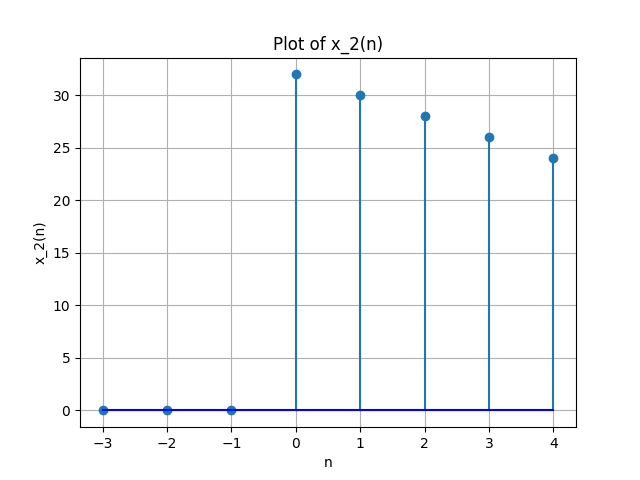
\includegraphics[width=10cm, height=6cm]{graph_2}
\captionsetup{Graph:2 $x_2(n)$ vs n }
\label{graph:3}
\end{figure}

\vspace{0.05cm}
\item[1)] 
\textbf{Z-Transform of $x_2(n)$} :
Using \eqref{eq:3}\vspace{0.05cm}
\begin{align}
\sum_{n=-\infty}^{\infty}(x_2(0) -2n)u_{(n)}Z^{-n} =X_2(z)
\end{align}
For $X_2(z)$ 
\begin{align}
  \notag 34z(1-z)^{-1}-\\
\notag 34z((1-z))^{-1}-\\
       2z((1-z))^{-2}=X_2(z)
\end{align}

\item[2)] 
\textbf{Calculating $S_2(k)$ of $x_2(n)$} :
For calculating the sum , we use \eqref{eq:1}
\begin{align}
 S_2{(13)} = \dfrac{13}{2}(64+11(-2))\\
 S_2{(13)}= 286.
 \end{align}
 \item[3)]
 \textbf{Region of Convergence}
\vspace{0.05cm}
\begin{align}
    \lvert z\rvert  <  1 
    \end{align}

\vspace{1cm}
 
\vspace{0.5cm}
\item[(iii)]
-5 + -8 + -11 ... -230\vspace{0.05cm}
\vspace{0.2cm}

Here $x_3(0)$ = -5, $d_3$ = -3\vspace{0.05cm}
From \eqref{eq:2}
\begin{align}
-230= -5 -3n \\
n=75
\end{align}
For $x_3(n)$
\begin{align}
x_3(n) = x_3(0) + nd_3\\
x_{3(n)}=x_3(0) - 3n
\end{align}

\begin{figure}[!ht]   
\centering
\graphicspath{ {figs/} }
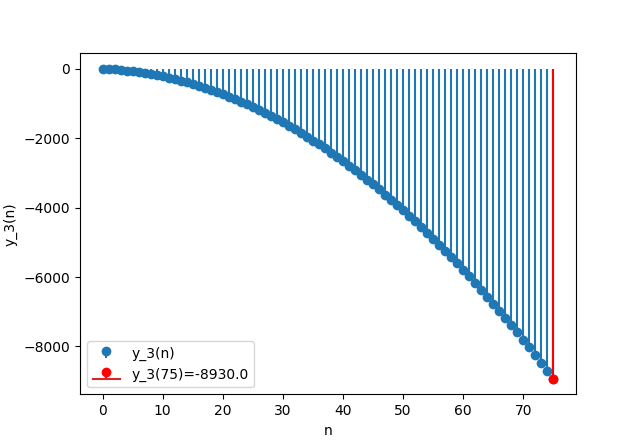
\includegraphics[width=10cm, height=6cm]{graph_3}
\captionsetup{Graph:3 $x_3(n)$ vs n }
\label{graph:4}
\end{figure}

\item[1)] 
\textbf{Z-Transform of $x_3(n)$} :
Putting $x_3(n)$ in \eqref{eq:3}\vspace{0.05cm}
\begin{align}
\sum_{n=-\infty}^{\infty}(x_3(0) -3n)u_{(n)}Z^{-n} =X_3(z)
\end{align}
For $X_3(z)$ , we use the same process as in (i) bit\vspace{0.05cm}
\begin{align}
  \notag -5z(1-z)^{-1}-\\
\notag 5z((1-z))^{-1}-\\
       3z((1-z))^{-2}=X_3(z)
\end{align}
\item[2)]
\textbf{Calculating $S_3(k)$ of $x_3(n)$} :
Using \eqref{eq:1} :\vspace{0.05cm}
\begin{align}
    S_3(76)=\dfrac{76}{2}(-10+(76-1)(-3))\\
   S_3(76)=-8930
    \end{align}
     \item[3)]
 \textbf{Region of Convergence}
\vspace{0.05cm}
\begin{align}
    \lvert z\rvert  <  1 
    \end{align}

\vspace{0.05cm}

  \vspace{1cm}
 \begin{center}
\begin{tabular}{ |c|c|c| } 
 \hline
 Symbols & Description & Values    \\
 \hline
  \small $d_i$ & \small Common Difference & 3.5, -2, -3\\
  \small $x_i(n)$ & \small Sequence  &  \scriptsize ($x_i(0)$ +$nd_i$)$u_{(k)}$\\
     \small $X_i(z)$ & \small Z-Transform of $x_i(n)$ & \scriptsize 2$x_i(0)(1-z)^{-1}+(d_i)z(1-z)^{-2}$ \\
     \small $S_i(k)$ & \scriptsize Sum of k-terms in $i^{th}$ series & \scriptsize $\dfrac{ku_{(k)}}{2}(2x_i(0) + (k-1)d_i)$\\
 \hline
\end{tabular}
\centering
\captionsetup{Table 1 : PARAMETERS , DESCRIPTIONS AND VALUES }
\end{center}
\end{enumerate}
\end{document}
